
%! program = pdflatex

\documentclass[12pt]{article}
\usepackage{amsmath}
\usepackage{natbib}
\usepackage{graphicx}
\usepackage{amssymb}
\usepackage{epstopdf}
\usepackage{float} % to keep the figures in place

\usepackage{color}
\newcommand{\cred}{ \color{red}}
\newcommand{\cgreen}{\color{green}}
\newcommand{\cblue}{\color{blue}}
\newcommand{\cmag}{\color{magenta}}
\newcommand{\bn}{\begin{enumerate}}
\newcommand{\en}{\end{enumerate}}
\newcommand{\bi}{\begin{itemize}}
\newcommand{\ei}{\end{itemize}}
\newcommand{\be}{\begin{eqnarray}}
\newcommand{\ee}{\end{eqnarray}}
\newcommand{\by}{\begin{eqnarray*}}
\newcommand{\ey}{\end{eqnarray*}}
\renewcommand{\labelenumi}{(\alph{enumi}) }
%
\usepackage[margin=2.2cm, includehead]{geometry}% see geometry.pdf on how to lay out the page. There's lots.
\geometry{letterpaper} % or letter or a5paper or ... etc
% \geometry{landscape} % rotated page geometry
%\bibpunct{(}{)}{;}{a}{,}{,}
%\setlength{\textwidth}{16cm}
%\setlength{\textheight}{21cm}
\def\nonumber{\global\@eqnswfalse}
\newcounter{parnum}
\newcommand{\N}{%
  \noindent\refstepcounter{parnum}%
   \makebox[\parindent][l]{\textbf{[\arabic{parnum}]}}\quad  }
% Use a generous paragraph indent so numbers can be fit inside the
% indentation space.
\setlength{\parindent}{1.5em}

% See the ``Article customise'' template for come common customisations

\date{}
%\date{} % delete this line to display the current date

%%% BEGIN DOCUMENT
\usepackage{Sweave}
\begin{document}
\Sconcordance{concordance:HW2.tex:HW2.Rnw:%
1 47 1 1 0 22 1 1 19 3 0 1 1 4 0 1 2 6 1 1 16 43 0 1 2 4 1 1 16 43 0 1 %
2 4 1 1 16 43 0 1 2 1 1}

%\large
%\maketitle
\newtheorem{thm}{Theorem}[section]
\newtheorem{cor}[thm]{Corollary}
\newtheorem{lem}[thm]{Lemma}
\newtheorem{prop}[thm]{Proposition}
\newtheorem{defn}[thm]{Definition}
\newtheorem{exam}[thm]{Example}
\newtheorem{qstn}[thm]{Question}

%%%
\newpage
\begin{center}
{\bf Homework 2 - STAT 511 - (Questions in R)}\\
Amal Agarwal
\end{center}
%==========================
\section*{Answer 1(c)}
\bn
\item The MLE calculated using the given data directly and the MLE obtained from the plot of likelihood function vs. p are respectively given as 
\begin{figure}[H]
\begin{Schunk}
\begin{Soutput}
[1] 0.5261122
\end{Soutput}
\begin{Soutput}
[1] 0.526
\end{Soutput}
\end{Schunk}
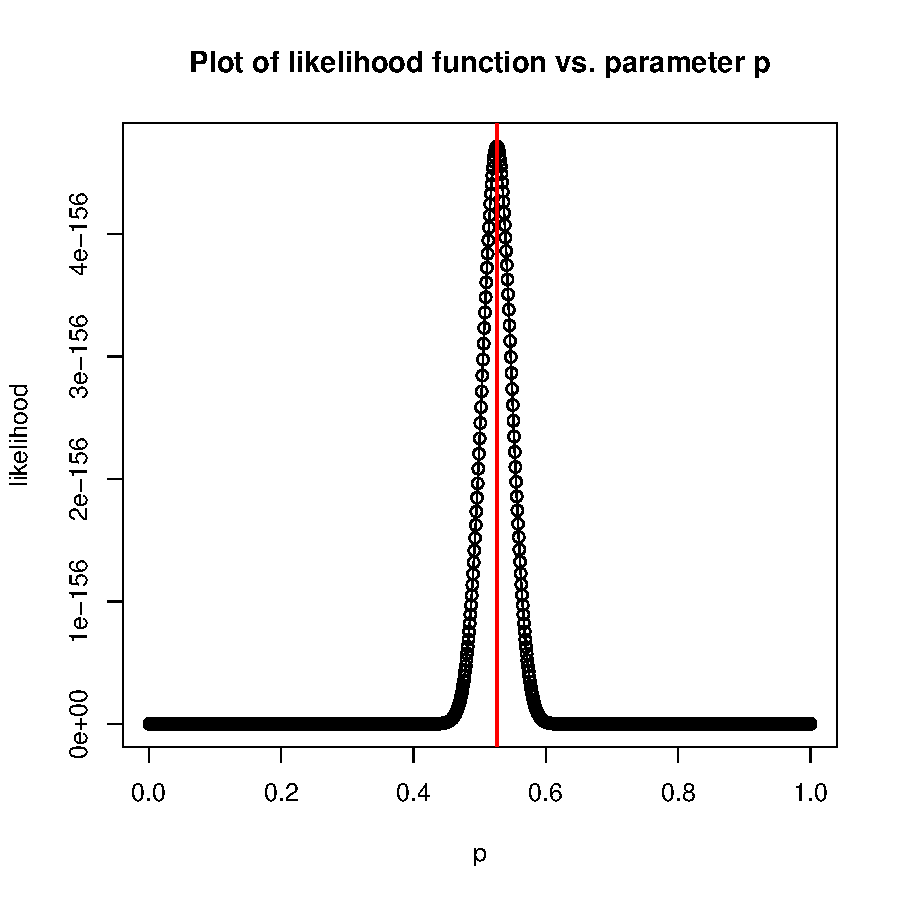
\includegraphics{HW2-001}
\end{figure}
\en

\clearpage
\section*{Answer 4(f)}

9 realizations of Y for $\sigma=\tau=1$ are given as:
\begin{Schunk}
\begin{Soutput}
            [,1]       [,2]       [,3]       [,4]        [,5]       [,6]
 [1,] -0.4223273 -1.1094835  2.1211835  2.2527498 -0.55625209 -2.0863166
 [2,]  1.3214603  3.0134466  3.4529991 -0.2971206 -1.25024432  0.9646389
 [3,]  0.3389225 -0.6492696 -1.4584103  0.5081058  0.09252057 -1.0705523
 [4,] -1.3691825  0.4085227 -1.6591660 -0.6597774 -0.46132689 -0.3277292
 [5,]  0.3868048  0.2391289  0.7882345 -0.3604249 -0.42000648  1.1945585
 [6,] -0.7123342 -1.3706632 -0.7240077 -1.2227066  0.20608792 -0.2261761
 [7,] -0.1131304 -1.0174985  1.3751599 -1.4101252 -1.19622533 -2.0222478
 [8,] -2.1905722 -1.3998160 -1.0668806 -1.9111053 -2.26915750 -1.6223337
 [9,] -0.2128252 -0.6807935 -2.2734067 -2.4226283 -1.62119061 -1.3955373
             [,7]       [,8]       [,9]       [,10]        [,11]       [,12]
 [1,] -0.19833473  0.6180953 -0.5993694 -0.51830728 -2.257335319 -2.39420766
 [2,] -0.51231958  1.2380695 -1.0564356  0.48888948  0.624604261 -1.07735691
 [3,] -1.64247504 -0.5023421 -0.2665972 -2.05685400 -0.283171808 -0.97521666
 [4,]  1.00116089  0.4390399  2.6666542  0.08550201 -0.003755992 -1.01163305
 [5,]  0.76893340  2.2133261  2.3867591  1.78293617  2.409815848  0.85708344
 [6,]  1.33072369 -1.7191783 -1.0990233 -0.69467394 -2.146054195  0.55552431
 [7,] -1.53935085 -1.0696641  0.3852306 -1.16578077 -0.925349605 -0.06995538
 [8,] -2.29935606 -1.0733085 -1.8748946  0.98537601  0.512407310 -0.16711320
 [9,] -0.04864026  0.9962093 -1.2060335  0.84319089 -1.362717305 -0.50076357
            [,13]       [,14]      [,15]       [,16]       [,17]      [,18]
 [1,] -0.97542530  0.80920050  0.5595841 -0.96241531 -0.99926054  1.5784529
 [2,] -0.96090648  1.40804879 -0.6225306  0.18782654 -1.34384158  1.8038887
 [3,] -1.71588713 -2.43264982 -1.9948680 -1.57174039  0.47492913  1.1057876
 [4,] -0.83747303  0.06683405  1.6604521 -0.77098751  1.41976354  1.1422756
 [5,]  1.60522132 -1.33721502 -0.5809175 -0.76107591 -1.09955180  2.4308274
 [6,]  1.52049472  2.28961448  1.6989177  2.15260723  3.03585706 -1.4781663
 [7,] -1.41004810 -2.41648473 -3.9617433  0.83176613  1.40379824  2.0877839
 [8,]  0.51986159  0.28792900 -0.5077620 -0.05525141  1.52236693 -1.0088625
 [9,] -0.01509715  0.25031860 -0.8695980 -0.76022502 -0.06050135  0.2379168
            [,19]      [,20]
 [1,]  0.07855636  1.4974453
 [2,] -0.68882157  0.6113622
 [3,]  0.63879683  0.1605124
 [4,]  0.81903400  0.4644464
 [5,]  0.50713328  1.5633754
 [6,]  1.43890947  0.1470442
 [7,]  1.54547229  1.8087092
 [8,]  1.10232287 -0.6447887
 [9,]  0.27146306  0.5494226
\end{Soutput}
\end{Schunk}

\clearpage
\section*{Answer 4(g)}

9 realizations of Y for $\sigma=10, \tau=1$ are given as:
\begin{Schunk}
\begin{Soutput}
            [,1]       [,2]       [,3]        [,4]         [,5]        [,6]
 [1,] -2.5513010  -2.316634  12.662578  24.3306636   9.05057571  14.7473057
 [2,] -8.2367924  -1.917888  -4.828586 -23.6764489  -7.80123846  -6.9166459
 [3,]  8.4347853  23.749706  -2.314998   8.4509041   7.64363709 -11.9844496
 [4,] -0.2215285 -15.514879 -14.315121 -19.1502604  -0.04553649   0.2453858
 [5,] 10.0112567 -19.110789   1.754514   2.8366588  -4.22127500  -4.7733345
 [6,]  3.2206667   2.873831 -13.131522 -12.1566102  -6.07536055   2.8402956
 [7,] 12.9655583   1.981036   5.739943  -5.0467873  11.80965271   8.2798198
 [8,] 10.0395260  -3.195844  -1.012456  18.1143218 -15.14804528   2.1848376
 [9,]  6.1032226   3.733907   6.294149  -0.9632901  -6.65902307  -4.4110771
            [,7]         [,8]       [,9]       [,10]      [,11]       [,12]
 [1,]  -7.784228  -2.35401042 13.9527102   0.4883518 -15.238151  11.6069763
 [2,]  -2.770664 -24.57737350 -3.1319825  -1.7604930 -12.765102   3.0638096
 [3,]  -1.925012   2.34864595 -4.8930875 -10.5674625   7.349630  -8.6336352
 [4,]   5.267098   2.81937508 12.1223109  -1.3935557 -14.516335  -4.2431572
 [5,]   6.864818  -9.18957157 -4.9626759  10.3821740   5.504470  -0.4014347
 [6,]  -7.251231 -15.51127357  6.5171215  13.6746915 -10.949198 -12.3829077
 [7,]   1.963400  -7.64477037  3.1937701   1.3500925   6.971114   8.0308204
 [8,] -10.869317 -11.86382853  0.5441963  -4.8180018   3.325156 -12.2670748
 [9,]  -3.785653  -0.04952326 15.2032020   9.1258790  -5.107511   3.2356755
           [,13]       [,14]      [,15]      [,16]      [,17]       [,18]
 [1,]  11.460001  -1.5549742   1.617165  6.2812892   7.510202   0.8229973
 [2,]  10.687142   2.6548277 -18.414406  0.2605695   1.245281  16.5101514
 [3,] -10.128065  16.0523659  11.186434 -5.7164004  -6.955001 -12.6235151
 [4,]   1.208623  10.9800861  11.650455 -4.2775041   3.917240   1.4951379
 [5,]  10.658542  -4.9027349  -2.091414  3.6058132 -16.406144  -0.6328887
 [6,]  -1.760053 -11.5670894 -12.422124 11.2988411   9.916571   2.7226389
 [7,]  -5.635450  -6.9360953   0.889747 -2.1155104  10.939074   7.7077347
 [8,]  -8.708915   0.6655690  17.450822  5.3759303 -15.050965  -1.3613525
 [9,]  -6.558134  -0.9757124  -4.273851 13.8069407   9.059201  -8.6330048
            [,19]      [,20]
 [1,] -6.20556227   3.742400
 [2,]  3.27372456  -1.746197
 [3,] -0.14517150  -7.696521
 [4,] 12.11482871  -7.103939
 [5,] 17.11971306   4.317644
 [6,]  4.02312785 -17.146630
 [7,]  0.04524416  -3.085935
 [8,] 14.22404381 -12.950097
 [9,] -7.00376585 -13.090150
\end{Soutput}
\end{Schunk}

\clearpage
\section*{Answer 4(h)}

9 realizations of Y for $\sigma=1, \tau=10$ are given as:
\begin{Schunk}
\begin{Soutput}
            [,1]        [,2]       [,3]       [,4]       [,5]        [,6]
 [1,] -13.667589 -20.2679075 -13.821877 -11.778836 -11.851648 -18.3474863
 [2,]   7.306048   4.9708094  10.219602   4.018004   8.649167   9.1065305
 [3,]  14.414489  17.7805264  10.442602  16.484026  15.879542  16.0009474
 [4,]  -7.719294  -4.3987747  -5.286546  -8.839495  -4.237285  -6.9149124
 [5,]  -2.981393  -3.4853579  -4.179148 -10.606244  -8.609855 -16.4817922
 [6,]   7.815893   2.1635104   8.224721   5.778912   7.135026   1.2056390
 [7,]   7.091315  14.1819368  17.438183  13.836574  10.240981   8.5511560
 [8,]  -3.612980  -0.5307973   2.521473  -3.185597   3.043660  -0.7187022
 [9,]  11.307301  12.4323746  16.789825  10.427438   4.832755   9.7649428
            [,7]       [,8]       [,9]       [,10]      [,11]      [,12]
 [1,] -17.825847 -10.165936 -11.562783 -14.6571791 -12.259852 -8.8073447
 [2,]  14.251974  16.572705  16.878073   9.4348326   3.600552  4.7133545
 [3,]  17.579080  10.586082  10.218731   9.3814930   4.665714 -3.0526236
 [4,]  -7.452400  -5.292886  -1.502365   0.1417718  -2.566104  6.2947086
 [5,]  -5.395341  -7.346215   1.051313   0.5514113   5.691520 12.5065215
 [6,]   5.372219   4.535731   3.258519  -0.8432053   5.782016 10.0560020
 [7,]   8.078930   6.450827   5.121730   7.4873054  15.364846  8.7942666
 [8,]   1.249173  -2.032297   3.940669   4.0918659  -3.255997  3.0575798
 [9,]   9.047663   7.216445   2.951823   6.1343592   1.234888  0.6564199
          [,13]     [,14]     [,15]      [,16]       [,17]       [,18]
 [1,] -7.799941 -5.797913  2.137496  8.5931734  12.0705614  11.0709355
 [2,]  3.461371  2.371494  5.480445  2.8775672   7.8617883   8.8397168
 [3,] -3.161658 -4.717086 -1.165675 -4.8300884 -10.3055468 -10.6710789
 [4,]  7.798152 13.132047  8.841115  8.2182973   0.4587017  -0.4063861
 [5,] 16.752658 12.016115  7.985354  6.9298565   2.0320159  -4.9507307
 [6,] 11.316698 16.743215  9.168340  8.3317196  10.7674784   9.0062679
 [7,]  6.914647 10.420642 10.069361  2.5249686   6.0893319   3.2632721
 [8,] -1.881671  1.644230 -1.586332  0.9424158 -10.5051912  -7.2176767
 [9,]  5.074168  6.731777 11.577223 16.6404653  11.3576468  21.0202827
           [,19]      [,20]
 [1,]  11.948764  10.995526
 [2,]   3.335023   5.914412
 [3,] -11.706268 -12.651138
 [4,]  -2.602530   1.423212
 [5,] -10.450468  -7.200422
 [6,]  11.352160  14.211639
 [7,]   8.927637  10.768516
 [8,] -13.059372 -15.353311
 [9,]  23.147844  22.728977
\end{Soutput}
\end{Schunk}

\end{document}
